%\anto{to be sent to: Journal of the European Mathematical Society?}

\section{Introduction}
Gelfand duality \cite[\S IV.4]{johnstone82stone} is a famous result in operator algebra establishing that the category of (unital) commutative $C^*$-algebras with $*$-homomorphisms is contravariantly equivalent to the category of compact Hausdorff spaces with continuous maps.
Together with the Riesz--Markov--Kakutani representation theorem
\cite[Theorem 2.14]{rudin1987analysis} --- which ensures that regular Borel probability measures on a compact Hausdorff space $X$ bijectively correspond to states on $C(X)$, i.e., completely positive unital (\cpu) functionals --- this perspective has motivated the adoption of $C^*$-algebras as a natural framework for noncommutative probability.
In recent years, Furber and Jacobs~\cite{furber_jacobs_gelfand} have further supported this adoption by establishing a \emph{probabilistic} Gelfand duality: \cpu maps between (unital) commutative $C^*$-algebras correspond to \emph{continuous} Markov kernels between compact Hausdorff spaces. 
Crucially, however, although disintegration of measures (or, in more naive terms, ``generalized Bayes' rule'') yield Markov kernels, it rarely produces continuous ones.

To overcome this limitation, one generally resorts to von Neumann algebras, often described as ``noncommutative measurable spaces''.
While this slogan is well motivated, it obscures an important distinction:
commutative von Neumann algebras are ``blind to null sets'' because their elements are \emph{equivalence classes} of random variables (modulo almost-everywhere equality).\footnote{A genuine Gelfand--type duality for von Neumann algebras requires a substantial revision of the notion of measurable space; see \cite{pavlov2022duality}.}
Formally, commutative von Neumann algebras correspond to measure algebras, i.e.\ complete Boolean algebras obtained by quotienting $\sigma$-algebras by null sets.

This might initially seem like a harmless technicality, but it has undesirable consequences.
For instance, one may wish to treat the Lebesgue measure on $\bbR$ together with delta measures.
However, singleton sets are null for the Lebesgue measure, so quotienting by null sets erases the information carried by individual points.

An approach tailored to measurable spaces was proposed by Tobias Fritz and the second author in \cite{fritz2025categories}.
In that work, the tentative noncommutative analogue of measurable spaces is given by \emph{\cstars{}s}, i.e.\ monotone $\sigma$-complete \cstar{}s~\cite{saito15monotone}.\footnote{Preliminaries on \cstars{}s are provided in \cref{sec:preliminaries}.
	For now, it suffices to recall that the standard morphisms between \cstars{}s are the \emph{$\sigma$-normal} maps.}
This proposal is supported by a Gelfand--type duality: assigning to every measurable space $X$ the commutative \cstars{} $\Linf(X)$ of bounded measurable functions yields an adjunction.
While this is not an equivalence in full generality, it restricts to one on standard Borel spaces and, beyond second-countability, on Baire measurable spaces~\cite[\S 4.2]{fritz2025categories}.
Moreover, the corresponding probabilistic morphisms, namely $\sigma$-normal \cpu{} maps, are closely related to positive operator-valued measures (POVMs).\footnote{This connection will also reappear in the present work; see \cref{sec:sigmaCP}.}
 
The present work builds on these developments.
The main theorem, which underlies the rest of the paper (see \cref{fig:secdep}), shows that the forgetful functor $U\colon \SigmaC \to \Calg$ from the category of \cstars{}s with $\sigma$-normal $*$-homomorphisms to the category of \cstar{}s with $*$-homomorphisms is \emph{monadic} (\cref{sec:monadic}). 
Roughly speaking, this means that \cstars{}s can be thought of as "algebras over \cstar{}s", and the rest of the paper exploits this description to ensure a number of consequences that are also of interest to readers less familiar with category theory. 
Though we will detail these findings below, we briefly mention that we will be able to describe \scpu{} maps via a universal property and moreover equip \cstars{}s with a tensor product. 
The adopted categorical methods uncover the conceptual unity underlying these results, which would otherwise require separate functional-analytic justifications.
\begin{figure}[ht]
	\centering
	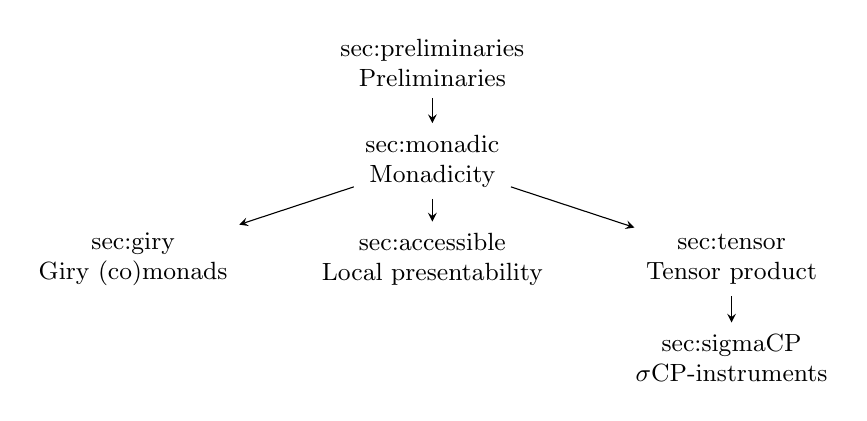
\begin{tikzpicture}[x=3.8cm,y=1.25cm,
			every node/.style={align=center,font=\small,inner sep=4pt},
			>=stealth]
		\node (preliminaries) at (0,0)
			{\cref{sec:preliminaries}\\Preliminaries};
		\node (monadicity) at (0,-1)
			{\cref{sec:monadic}\\Monadicity};
		\node (giry) at (-1,-2)
			{\cref{sec:giry}\\Giry (co)monads};
		\node (accessible) at (0,-2)
			{\cref{sec:accessible}\\Local presentability};
		\node (tensor) at (1,-2)
			{\cref{sec:tensor}\\Tensor product};
		\node (instruments) at (1,-3)
			{\cref{sec:sigmaCP}\\$\sigma$CP-instruments};
		\draw[->] (preliminaries) -- (monadicity);
		\draw[->] (monadicity) -- (giry);
		\draw[->] (monadicity) -- (accessible);
		\draw[->] (monadicity) -- (tensor);
		\draw[->] (tensor) -- (instruments);
	\end{tikzpicture}
	\caption{Section dependencies, with transitive arrows omitted.}\label{fig:secdep}
\end{figure}

The corresponding monadicity result for von Neumann algebras was established by Furber~\cite{furber2024monad}.
An important distinction is that Furber proves monadicity only for normal $*$-homomorphisms, whereas here we show it holds both for $\sigma$-normal $*$-homomorphisms and for $\sigma$-normal \cpu{} maps (\cref{rem:monadic_cpu}). 
In fact, the present result can be seen as a refinement. 
As observed in \cref{rem:monadicity_W}, Furber's theorem together with \cref{thm:U_monadic} yields that $\Walg \to \SigmaC$, where $\Walg$ denotes the category of von Neumann algebras with normal $*$-homomorphisms, is monadic as well. 
In particular, we obtain a tower of monadic functors
\[  
\Walg \longrightarrow \SigmaC \longrightarrow \Calg
\]
of which the present paper supplies the middle step.

Given the categorical and operator-algebraic nature of this paper, we now describe the results from both perspectives, in order to provide conceptual insight to readers from either community.

\subsection*{From a categorical viewpoint}
\begin{itemize}
	\item Using the fact that $\Calg$ (and its subcategory of commutative \cstar{}s) has a comonad describing \cpu{} maps as coalgebras, we establish the existence of an analogous comonad on $\SigmaC$, describing $\sigma$-normal \cpu{} maps as coalgebras (\cref{sec:giry}).

	      Moreover, the comonad for commutative algebras extends the \emph{Giry monad} of \cite{giry82probability} when restricted to Baire measurable spaces \cite[\S4.2]{fritz2025categories}, which generalize standard Borel spaces beyond second countability.
	\item $\SigmaC$ is locally $\aleph_1$-presentable, and the forgetful functor $U\colon \SigmaC \to \Calg$ is accessible (\cref{sec:accessible}).
	\item $\SigmaC$ is a symmetric monoidal category, and the same holds when extending to $\sigma$-normal \cpu{} maps (\cref{sec:tensor}).
	\item The monoidal category is not closed, but a property similar to monoidal closure holds when one object is commutative (\cref{sec:sigmaCP}).
\end{itemize}
\subsection*{From an operator-algebraic viewpoint}
\begin{itemize}
	\item The \cstar{} of continuous functions over the state space and the universal \cstar{}~\cite[Proposition 8]{kirchberg1998Cstarfromoperator} ensure the existence of \cstars{}s having analogous universal properties (\cref{sec:giry}).

	      Unfolding this, for any \cstars{} $\A$ there exists a unique \cstars{} $\mathcal{P}(\A)$ such that every $\sigma$-normal \cpu{} map $\A \to \B$ factorizes as
	      \[
		      \xymatrix{\A\ar[r]\ar[d] & \B\\ \mathcal{P}(\A)\ar@{-->}[ru]}
	      \]
	      where $\mathcal{P}(\A)\to \B$ is a $\sigma$-normal $*$-homomorphism.
	      Similarly, there is a \emph{commutative} \cstars{} $\mathcal{S}(\A)$ when the universal property is tested only on commutative $\B$.
	\item Roughly speaking, each \cstars{} is built from a small set of `$\aleph_1$-compact' \cstars{}s by taking direct sums and quotients (\cref{sec:accessible}).
	\item \cstars{}s have a tensor product $\kocktensor$ obtained by extending the maximal tensor product $\otimes$ on \cstar{}s (\cref{sec:tensor}).
	      In particular, morphisms of type $\A \kocktensor \B \to \C$ are in bijective correspondence with those of type $\A \otimes \B \to \C$ which are \emph{bi-$\sigma$-normal}, i.e.\ separately $\sigma$-normal in each variable (\cref{def:bisigmanormal}).
	      This resembles the universal property of the binormal tensor product for von Neumann algebras (compare \cite[Proposition 2.1]{okamura2015measurement} with \cref{thm:tensor_shom}), where ``binormal'' means precisely ``normal on each tensor factor''.
	\item The discussion of \cite{okamura2015measurement} regarding \emph{CP-instruments} in the context of von Neumann algebras can be reformulated for \cstars{}s (\cref{sec:sigmaCP}). 
	Below, we offer some insights on this notion and our contributions to this matter.

	CP-instruments are due to Davies and Lewis~\cite{davies1970operational}, who introduced them to treat repeated measurements of \emph{continuous} observables without commutation hypotheses. Ozawa~\cite{ozawa1984quantummeasuring} established their correspondence with measuring processes in the Hilbert space setting. 
	The underlying intuition is that every abstract instrument admits a concrete dynamical realization in much the same way that the GNS construction realizes abstract states on \cstar{}s as concrete vector states in a Hilbert space representation.

	An extension to arbitrary von Neumann algebras was provided in \cite{okamura2015measurement}, where however dynamical realizations are not always ensured. 
	To see where difficulties arise, we mention that this realization requires two steps: first, rewriting CP-instruments using a tensor product; second, verifying whether this tensor product extends to a von Neumann algebra. While the former can be proven in full generality (\cite[Proposition 3.3]{okamura2015measurement}), the latter requires an additional property called the ``normal extension property''.

	In this paper, \cref{thm:sigmaCPinstruments} establishes both of the steps highlighted above by weakening normality (proper to von Neumann algebras) to $\sigma$-normality (proper to \cstars{}s). 
	Crucially, no additional property is required.
\end{itemize}
\begin{paperacknowledgments}
We are grateful to Tallinn University of Technology and Pawel Sobocinski for inviting the second author to visit the institute, thereby sparking the collaboration between the two authors that eventually led to this manuscript.
We thank Tobias Fritz for his comments and insights on a draft of this paper.
We also thank Robert Booth, whose interest inspired the developments of \cref{sec:sigmaCP}.
\begin{paperfunding}
{The first author gratefully acknowledges the support of Tallinn University of Technology and of the Estonian Research Council grant~PRG3215.}
\end{paperfunding}
AI tools (particularly, Claude and Gemini Notebook) were employed to polish writing and ideas; their technical contributions remained marginal and were always verified by the authors, who take full responsibility for any errors in the manuscript.\footnote{Almost certainly, such errors will have a human fingerprint anyway.}
\end{paperacknowledgments}
